\chapter{Experiencia de Desarrollo de OpenSITEM}

Como se ha mencionado, openSITEM es centrado en la arquitectura y guiado por casos de uso. Tanto el Director de Proyecto como los equipos de trabajo temporales, están comprometidos con la tarea de generar un aplicativo funcional que esté alineado - de manera emergente, con las vistas arquitectónicas planteadas.

Con el método definido, los artefactos se construyen de manera iterativa e incremental. El ``orden'' en el que aquí se muestra no implica una secuencia de actividades pues no en pocas ocasiones, abordar la disciplina de \textit{Modelado de Dominio} se realiza a continuación de - o en paralelo a, un taller de requisitos y dicho taller surge de una nueva restricción detectada al momento de despliegue. Esta capacidad de adaptación al cambio es lo que ha permitido que openSITEM vaya realizando la transición desde un aplicativo específico a una suite escalable - potenciada por la arquitectura de federación de aplicaciones, orientada a servicios que está implementando.

En la implementación de cada uno de los módulos de openSITEM se siguen las fases contempladas en el Proceso Unificado\footnote{Inicio, elaboración, construcción y transición.} y se desarrollan flujos de trabajo en las disciplinas básicas de:

\begin{itemize}
\item Requisitos.
\item Arquitectura.
\item Elaboración.
\item Pruebas.
\item Despliegue.
\end{itemize}

A partir de iteraciones continuas por las diferentes disciplinas se refinan constantemente los modelos y se presentan resultados que permiten medir los avances, así como comprobar los niveles de calidad y la validez tanto de los entregables como del método empleado. 

\section{Modelo de Requisitos}

Un requisito es una declaración explícita y aceptada de la funcionalidad que un usuario espera del sistema. Dicha declaración debe ser coherente con el objeto de estudio de openSITEM, respetando siempre los principios normativos y de propiedad intelectual. Cada requisito se plasma en un documento denominado Caso de Uso, el cual describe un conjunto de escenarios de interacción del usuario con el sistema, con el propósito de obtener algo de valor.

\subsection{Declaración del Problema}

OpenSITEM es una propuesta de solución a los siguientes problemas:

\begin{itemize}
 \item La información de los estudios de campo no está estructurada, está dispersa, se ha perdido y es difícil de consultar y consolidar.
 \item El equipo de diseño de GITEM no cuenta con un mecanismo estándar para caracterizar los componentes de las redes de eSalud.
 \item No es posible determinar el valor de un nodo dentro de una red de eSalud.
 \item No existe capacidad de análisis multitemporal para determinar la valides de la categorización de nodos de una red de eSalud.
\end{itemize}

\subsection{Responsabilidades del Sistema}

El sistema debe contribuir a que los investigadores:

\begin{itemize}

\item Caractericen nodos con potencialidad de pertenecer a redes de eSalud.
\item Creen instancias de nodos a partir de la información de los estudios de campo que desarrollo el grupo.
\item Comparen nodos de la misma categoría para definir cual tiene mayor valor relativo.
\item Consulten catálogos especializados en cada categoría de nodos.
\item Definan modelos de categorías de nodos.
\item Evalúen la potencialidad de un nodo para pertenecer a una red de eSalud.
\end{itemize}


\section{Alcance}

OpenSITEM no implementa todo el modelo del requisitos. Los módulos desarrollados son prototipos funcionales que sirven de guía para el desarrollo y evolución posterior de la solución. Si relacionamos esto con el proceso OpenUP, el grupo en la fase III alcanza el final de la fase elaboración.

\section{Definición de actores}

El sistema es manejado por varios tipos de usuarios, cada uno con características específicas. Este tratamiento especial tiene que ver con el mantenimiento de la integridad de la información, la cual solo puede ser gestionada por un grupo selecto de usuarios. 

Algunos actores esperados en el openSITEM son:

\begin{itemize}
\item Administrador.
\item Consultor.
\item Especialista Médico.
\item Profesional TIC.
\item Usuario General.
\end{itemize}

Cada uno de ellos con las características mostradas en el anexo \ref{modelo_requisitos}.

\section{Casos de uso}

Los requisitos funcionales son declarados con diferente nivel de detalle empleando casos de uso, diagramas de comportamiento y de interacción. Al caracterizar una interacción por medio de un caso de uso se espera tener información acerca de:

\begin{itemize}
\item Nombre del Caso de Uso
\item Objetivo que se logra al ejecutarse el caso de uso.
\item Código que lo identifique unívocamente dentro del banco de artefactos.
\item Actores que intervienen al desarrollarse el caso de uso.
\item Casos de uso con los que está relacionado.
\item Precondiciones.  El estado del sistema que debe asegurarse antes de que el caso de uso inicie. Debido a que es responsabilidad del sistema no se verifica en el caso de uso.
\item Postcondiciones. Las características y estado del sistema una vez se haya terminado el caso de uso.
\item Flujo de Tareas. Flujo principal y flujos alternativos de las actividades que se suceden para lograr la funcionalidad deseada. Se debe mantener claridad en el modelo por lo que se recomienda utilizar diferentes artefactos para los flujos alternativos cuando esto lo amerite.
\end{itemize}

La tabla \ref{casouso}, muestra el flujo principal del un caso de uso de openSITEM.

\begin{table}
\begin{center}
\begin{tabular}{|l|p{10cm}|}
\hline
\textbf{Caso de Uso}&\\
\hline
Nombre & Evaluar Capacidad de un Nodo\\
\hline
Objetivo & El actor asigna un valor y un diagnóstico a un nodo que da cuenta de la capacidad que tiene dicho nodo de pertenecer a una red de eSalud .\\
\hline
Código Interno & UC-GENERAL-XXXX \\
\hline
Actores & Consultor\\
\hline
Precondiciones & El nodo se encuentra registrado en el sistema en estado ACTIVO.\\
\hline
Flujo Básico & 1. El Consultor selecciona el nodo que desea evaluar.\\
& 2. OpenSITEM presenta los datos relacionados con el nodo\\
& 3. El Consultor revisa el historial de valoraciones del nodo.\\
& 4. El Consultor revisa el valor de los atributos del nodo. \\
& 5. El Consultor valora el nodo.\\
& 6. El Consultor argumenta la valoración a través de un diagnóstico.\\
& 7. OpenSITEM guarda los datos de la valoración.\\
& 8. OpenSITEM envía una notificación de la valoración a los interesados.\\
\hline
Postcondiciones & Se agregó una valoración argumentada al sistema.\\
\hline
Casos de uso relacionados&Consultar Historial de Valoración de Nodo\\
\hline
\end{tabular}
\caption{Caso de Uso Evaluar Capacidad de Nodo}
\label{casouso} 
\end{center}
\end{table}

El modelo actual tiene 80 casos de uso principales definidos\footnote{No se incluyen casos de uso implementados en aplicaciones conexas.} y más de 230 flujos alternativos - los más relevantes incluidos en el anexo \ref{modelo_requisitos}. Con esto se concreta los requerimientos de más alto nivel definido por el grupo GITEM. Se recalca que el grueso de ellos aún no se han desarrollado por lo que se probablemente el modelo se adapte a medida que se progresa en la construcción.

\section{Arquitectura}

Los requisitos son insumo para modelar los elementos del sistema y sus relaciones. El equipo de desarrollo se ha apoyado en diferentes diagramas de estructura y de comportamiento e interacción para describir la estructura y el comportamiento del sistema. El anexo \ref{modelo_analisis} corresponde a las vistas de la arquitectura que contienen los elementos más interesantes para diferentes partes del sistema. Como puede observarse en dicho anexo, se han aplicado varios patrones de diseño \footnote{Basados en General Responsibility Assignment Software Patterns (GRASP) y GoF} \cite{larman2003}, \cite{gamma1994} especialmente se presta atención a mantener los principios de:

\begin{itemize}
\item Alta Cohesión
\item Bajo Acoplamiento
\end{itemize}

Asignando responsabilidades teniendo en cuenta:
\begin{itemize}
\item Experto en Información.
\item Controlador
\end{itemize}

En la figura \ref{secuencia}, se muestra el diagrama de interacción correspondiente a la realización del caso de uso no esencial de registrarse en el sistema.

\begin{figure}
 \centering
 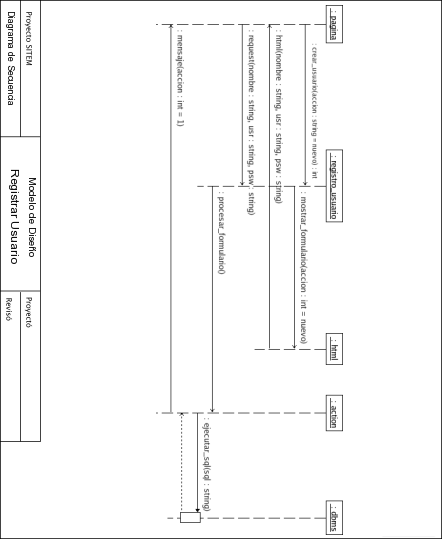
\includegraphics[width=156mm, height=156mm]{secuencia.png}
 \caption{Realización del Caso de Uso registrarse en el Sistema}
 \label{secuencia}
\end{figure}


\section{Modelo de Implementación}

El conjunto de diagramas del Anexo \ref{modelo_analisis} brinda la información fundamental para el modelo de implementación. En el openSITEM se agrupan los diferentes componentes en la jerarquía de carpetas mostrada en la figura \ref{carpetas_sitem}.

Cada una de las carpetas contiene los ficheros de código fuente del producto:

\begin{itemize}
 \item \textbf{Clases:} Contiene los archivos en PHP que implementan las clases. 
\item \textbf{Funciones:} Grupo de funciones en JavaScript para la validación de información en el nodo de usuario. En la actualidad la fase IV contempla complementar esta aproximación con la utilización de AJAX.
\item \textbf{Configuración:} Alberga el archivo \textit{config.inc.php} que guarda las variables de ingreso a la base de datos. Dichas variables se encuentran codificadas de acuerdo al algoritmo que se seleccione (o implemente) desde la clase \textit{codificar}.
\item \textbf{Bloques:} Agrupa el código fuente de cada bloque desarrollado en el openSITEM. Un bloque se define como una unidad de funcionalidad independiente que puede utilizarse en cualquier página.
\item \textbf{Estilo:} Información acerca de los parámetros generales de estilo - tamaño de fuente, color de bordes, fondos, colores de letras, etc; para diferentes componentes del openSITEM. La modificación o inclusión de parámetros afectará la interfaz global del sistema. Actualmente los estilos en el openSITEM se basan en hojas de estilo CSS.
\item \textbf{Gráficos:} Todos los archivos gráficos usados en el proyecto.
\item \textbf{Documentos:} Carpeta inicialmente vacía que se utiliza para guardar los archivos que los usuarios carguen a través del protocolo HTTP. Por seguridad se recomienda que esta carpeta se encuentre fuera del directorio en donde se encuentra instalada la aplicación.
\item \textbf{Instalar:} Contiene el instalador del producto. Esta carpeta debería ser retirada una vez el sitio se encuentre en producción.
\item \textbf{Desarrollo:} Con varios scripts que facilitan la tarea de desarrollo y adaptación de bloques en el sistema. Estos scripts se han construidos pensando en plataformas de desarrollo y prueba por lo que se supone no debe encontrarse en plataformas de producción.
\end{itemize}

En todo caso, durante el proceso de instalación se puede - y recomienda; asociar nuevos nombres a las carpetas por lo que en teoría ningún desarrollo basado en el openSITEM que esté en etapa de producción debería tener nombres de carpetas conocidos.

\begin{figure}
 \centering
 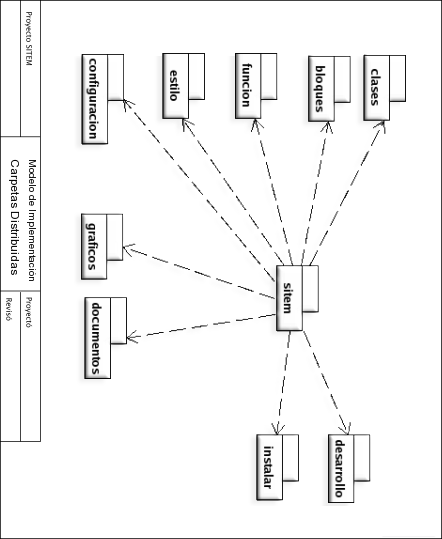
\includegraphics[width=156mm, height=156mm]{carpetas.png}
 \caption{Carpetas que se distribuyen con el openSITEM}
 \label{carpetas_sitem}
\end{figure}

\section{Acerca de la Seguridad en el Sistema}

Al tratarse de una aplicación web se tiene grandes retos con la seguridad. Se emplea como referencia el top 10 del proyecto OWASP\cite{owasp2017}, que para el año 2017 considera que los riesgos más importantes son: 

\begin{itemize}
  \item Inyección.
  \item Fallos en la Autenticación.
  \item Exposición de datos sensibles.
  \item Entidades externas XML.
  \item Fallos en el Control de Acceso.
  \item Fallos en la configuración.
  \item Cross-Site Scripting (XSS).
  \item De-serialización insegura.
  \item Uso de componentes con vulnerabilidades conocidas.
  \item Gestión y seguimiento ineficiente a los registros del sistema.
\end{itemize}

Para cada una de estos riesgos el equipo de desarrollo ha estudiado e implementado las técnicas y controles que la misma guía de la OWASP declara. La documentación del modelo de seguridad está siendo elaborada en el marco de una tesis de pregrado, la cual se encuentra en sus primeras etapas.

Como ejemplo, la figura\ref{desenlace} muestra la manera que OpenSITEM implementa un control sobre A2:2017, usando el gestor de sesiones de lado de servidor para generar un identificador aleatorio para cada una de las peticiones de página. Dicha técnica se asegura de crear cada cierto periodo de tiempo\footnote{Predefinido a 5 minutos} una llave única que garantiza un alto nivel de entropía en la cadena codificada - lo que implica que cada recurso tendrá un tiempo de expiración.

\begin{figure}
 \centering
 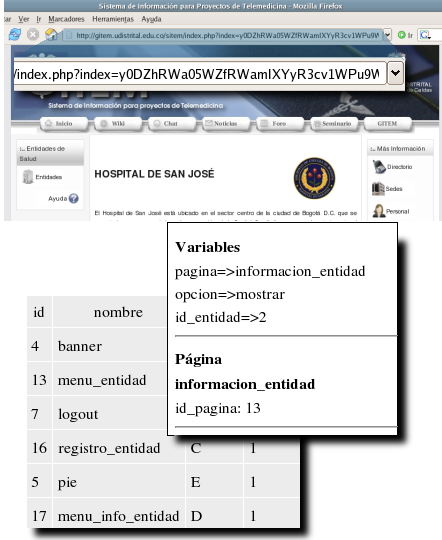
\includegraphics[width=80mm]{desenlace.png}
 \caption{URL encriptada. Con la herramienta \textit{Desenlace} el desarrollador puede descifrar los datos}
 \label{desenlace}
\end{figure}

En cuanto a la integridad de los datos se tiene un modelo de comparación de contenidos que se activa cada periodo de tiempo, el cual es programable; proponiéndose mantener una copia de respaldo verificada y avalada por el administrador. En caso de corrupción o pérdida de datos se mantiene una lista completa de los usuarios del sistema de hasta 1’000.000 de sesiones de tipo desplazamiento en donde el usuario más antiguo es descartado para la inclusión del nuevo cuando el tamaño asignado es completado, asegurándose el manejo eficiente de disco. 

Por ningún motivo se permite el acceso a sitios restringidos a usuarios que no hayan sido plenamente identificados en el sistema. En sitios críticos se hace una revisión de los datos de acceso guardados en cookies o se constata los datos de inicio de sesión. Se han evitado al máximo el uso de carácter comodín y todos los accesos a la base de datos son validados en su sintaxis. El openSITEM actualmente propone el uso de protocolos seguros tales como SSL.

Vale la pena destacar el uso de métodos de autenticación de usuario basado en sesiones y codificación de datos que permiten ofrecer un contenido personalizado de acuerdo al perfil de cada uno de los clientes del sistema.


\section{Modelo de Datos}

Dentro del proceso de desarrollo del openSITEM el modelado y elaboración del sistema de bases de datos es una de las partes fundamentales de la propuesta. Se ha venido estructurando el modelo de acuerdo a las necesidades de cada módulo en particular para garantizar la independencia entre ellos en cada una de las capas, incluyendo la de persistencia.

Dependiendo de las características de cada subsistemas se implementan o no políticas transaccionales. El modelo de seguridad en los datos hereda todos los elementos del servidor tales como bloqueos de puertos, ocultación de ventanas, manejo de sockets, etc; además, un esquema lógico de validación por conexiones persistentes complementa estas características.

El anexo \ref{modelo_datos} contiene los diagramas de clases que describen la arquitectura de datos del sistema y cada uno de sus subsistemas asociados. 

En la actualidad el openSITEM acepta bases de datos PostgreSQL, MySQL y ORACLE. La capa de persistencia del hilo principal se despliega sobre un servidor MySQL.


\section{Interfaz gráfica.}

De acuerdo a los diagramas conceptuales del portal GITEM y de openSITEM. Se han utilizado para la creación de las páginas los conceptos de diseño web enumerado por \cite{krug2014}, intentando evitar al máximo las páginas sobrecargadas de información. La navegación es guiada mediante enlaces, los cuales están agrupados temáticamente logrando una coherencia en el contenido. 

Los gráficos han sido optimizados y su inclusión es necesaria para dar ayuda visual al contenido basado en texto. Teniendo en cuenta que el openSITEM esta diseñado para interactuar permanentemente y por periodos prolongados de tiempo con el cliente, se han evitado deliberadamente la utilización  de componentes dinámicos. No obstante, el diseño no pierde atractivo ya que su implementación se fundamenta en bibliotecas de uso extendido.

Para reducir el tiempo de acceso al portal, sobre todo cuando se trabaja con conexiones lentas, se da la posibilidad en algunos subsistemas de descargar en formato PDF todo el contenido del grupo de páginas en donde se este ubicado.

\subsection{Arquitectura de la página}

Independiente del subsistema que nos encontremos las páginas siempre están compuestas por cinco secciones denominadas genéricamente con las letras A, B, C, D y E. En ellas se distribuyen los diferentes bloque que conforman la página en una arquitectura Top - Down. Las páginas que no tienen bloques en todas las secciones colapsan aquellas que no se utilizan para dar una impresión visual consistente. Las figuras \ref{secciones} y \ref{seccion_colapsada} muestran gráficamente el manejo de las secciones en cada página.

\begin{figure}
 \centering
 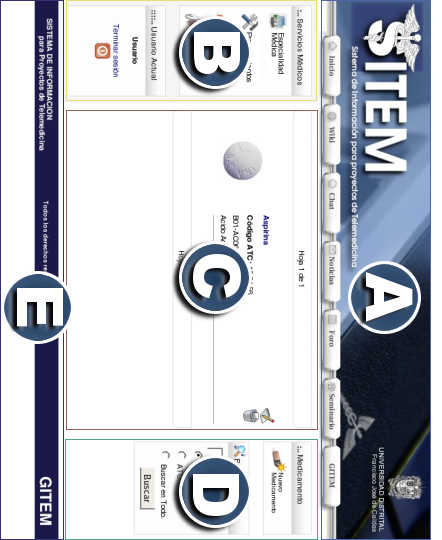
\includegraphics[width=156mm, height=156mm]{secciones.png}
 \caption{Arquitectura de una página en el openSITEM}
 \label{secciones}
\end{figure}

\begin{figure}
 \centering
 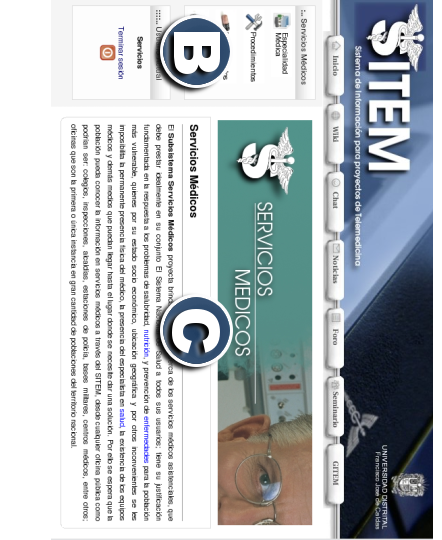
\includegraphics[width=156mm, height=156mm]{seccion_colapsada.png}
 \caption{Página del openSITEM en donde la Sección D se ha colapsado.}
 \label{seccion_colapsada}
\end{figure}

\section{Entregables del proyecto}

Los siguientes artefactos – documentos, son generados y utilizados por el proyecto. En el anexo \ref{entregables} se tiene extractos importantes de algunos de ellos.

\begin{itemize}
\item \textbf{Plan General de Trabajo}
\item \textbf{Modelo de Casos de Uso}. El cual especifica los requerimientos que debe cumplir el módulo de software y que en últimas constituye los contratos que éste, el módulo, tiene con actores externos. Este artefacto estará hecho en su totalidad usando el Lenguaje de Modelado Unificado. 

Dentro de este modelo se tienen dos vistas claras: la del negocio y la del sistema. El modelo de Casos de Uso del Negocio ilustra el ámbito del negocio que esta siendo modelado. El diagrama contiene actores del negocio y los servicio o funciones que ellos requieren del negocio. El modelo de casos de uso del sistema representa el ámbito de una aplicación. De esto se tiene que un solo modelo de casos de uso del negocio puede tener muchos Modelos de casos de uso asociados, donde cada modelo de casos de uso representa una única aplicación.

\item \textbf{Modelo de Objetos.} El cual describe la forma en que cada requerimiento – o contrato,  es cumplido. Establece las entidades internas, la información que intercambian y los flujos de trabajo que logran el cumplimiento de los requisitos. Los grafos correspondientes podrán incluir diagramas estáticos o interactivos expresados en UML.

\item \textbf{Glosario.} Que es el único artefacto válido de consulta para la terminología usada en el desarrollo del openSITEM. Ver el anexo \ref{glosario}.

\item \textbf{Visión.} Este documento define la visión del openSITEM. Es de todos el que marca las pautas conceptuales. 

\item \textbf{Especificaciones Adicionales.} Este documento captura los requisitos que no han sido incluidos como parte de los casos de uso y se refieren requisitos no-funcionales globales. Dichos requisitos incluyen: requisitos legales o normas, aplicación de estándares, requisitos de calidad del producto, tales como: confiabilidad, desempeño, etc., u otros requisitos de ambiente, tales como: sistema operativo, requisitos de compatibilidad, etc. 

\item \textbf{Prototipos de Interfaces de Usuario.} Se trata de prototipos que permiten al usuario hacerse una idea más o menos precisa de las interfaces que proveerá el sistema y así, conseguir retroalimentación de su parte respecto a los requisitos del sistema. Estos prototipos se realizarán como: dibujos a mano en papel, dibujos con alguna herramienta gráfica o prototipos ejecutables interactivos, siguiendo ese orden de acuerdo al avance del proyecto. Sólo los de este último tipo serán entregados al final de la fase de Elaboración, los otros serán desechados. Asimismo, este artefacto, será desechado en la fase de Construcción en la medida que el resultado de las iteraciones vayan desarrollando el producto final. 

\item \textbf{Arquitectura.} Este modelo establece la realización de los casos de uso en clases y pasando desde una representación en términos de análisis (sin incluir aspectos de implementación) hacia una de diseño (incluyendo una orientación hacia el entorno de implementación), de acuerdo al avance del proyecto.  Consultar el anexo \ref{modelo_analisis}.

\item \textbf{Modelo de Datos.} Previendo que la persistencia de la información del sistema será soportada por una base de datos relacional, este modelo describe la representación lógica de los datos persistentes, de acuerdo con el enfoque para modelado relacional de datos. Para expresar este modelo se utiliza un Diagrama de Clases (donde se utiliza un profile UML para Modelado de Datos, para conseguir la representación de tablas, claves, etc.). El anexo \ref{modelo_datos} contiene los artefactos más importantes del modelo de datos. 

\item \textbf{Modelo de Implementación.} Este modelo es una colección de componentes y los subsistemas que los contienen. Estos componentes incluyen: ficheros ejecutables, ficheros de código fuente, y todo otro tipo de ficheros necesarios para la implantación y despliegue del sistema.

\item \textbf{Modelo de Despliegue.} Este modelo muestra el despliegue la configuración de tipos de nodos del sistema, en los cuales se hará el despliegue de los componentes. Ver anexo \ref{modelo_despliegue} 

\item \textbf{Casos de Prueba.} Cada prueba es especificada mediante un documento que establece las condiciones de ejecución, las entradas de la prueba, y los resultados esperados. Estos casos de prueba son aplicados como pruebas de regresión en cada iteración. Cada caso de prueba llevará asociado un procedimiento de prueba con las instrucciones para realizar la prueba, y dependiendo del tipo de prueba dicho procedimiento podrá ser automatizable mediante un script de prueba. 

\item \textbf{Solicitud de Cambio.} Los cambios propuestos para los artefactos se formalizan mediante este documento. Mediante este documento se hace un seguimiento de los defectos detectados, solicitud de mejoras o cambios en los requisitos del producto. Así se provee un registro de decisiones de cambios, de su evaluación e impacto, y se asegura que éstos sean conocidos por el equipo de desarrollo. Los cambios se establecen respecto de la última baseline (el estado del conjunto de los artefactos en un momento determinado del proyecto) establecida. En nuestro caso al final de cada iteración se establecerá una baseline. 

\item \textbf{Plan de Iteración.} El conjunto de actividades y tareas se orden temporalmente y se le asignan recursos a corto plazo. Se realiza para cada iteración y en todas las fases. 

\item \textbf{Lista de Riesgos.} Este documento incluye una lista de los riesgos conocidos y vigentes en el proyecto, ordenados en orden decreciente de importancia y con acciones específicas de contingencia o para su mitigación. El anexo \ref{riesgos} contiene la declaración de los riesgos más importantes detectados en el proyecto así como estrategias para minimizarlos.

\end{itemize}